\section{Formalização do Problema}
\frame{
  \frametitle{Formalização do Problema}	
  \begin{block}{}
    \begin{figure}[H]
    \centering
    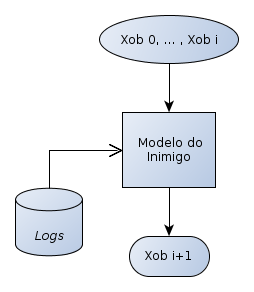
\includegraphics[scale= 0.35]{imgs/objetivo}
    \caption{Esquema inicial do problema}
    \end{figure}
  \end{block}  
  \begin{block}{}
    \begin{center}  
      Knowledge Discovery in Databases (KDD)
    \end{center}
  \end{block}
}

\frame{
  \frametitle{Formalização do Problema}
  \begin{block}{}
    \begin{figure}
      \centering
      \includegraphics[width=8.5cm]{imgs/campo_ssl}
      \caption{Estrutura da SSL}
    \end{figure}
  \end{block}
}

\subsection{Definições}

\begin{defi}[Corpo Rígido]
  Um corpo rígido $r$ é definido por dois subconjuntos disjuntos
  de parâmetros $r= \langle \hat{r}, \bar{r} \rangle$ em que:
  \begin{itemize}
    \item $\hat{r} = \langle \alpha, \beta, \gamma, \omega \rangle$,
    que são os parâmetros de estado mutáveis, respectivamente:
    posição ($\mathbb{R} ^{3}$), orientação ($\mathbb{R} ^{3}$),
    velocidade linear ($\mathbb{R} ^{3}$), velocidade angular
    ($\mathbb{R} ^{3}$)

    \item $\bar{r} :$ parâmetros imutáveis do corpo que descrevem sua
    natureza fixa e que permanecem constantes ao longo do curso de 
    planejamento.
  \end{itemize}
\end{defi}

  Exemplos de parâmetros considerados nesta modelagem imutáveis são:
  coeficiente de atrito estático e dinâmico, descrição $3D$ do corpo
  (por exemplo, por meio de um conjunto de primitivas $3D$), centro de
  massa no referencial do corpo, coeficiente de restituição,
  coeficiente de amortecimento linear e angular.

\begin{defi}[Bola]\label{def:bola}
  Bola é um corpo rígido $\hat{b}$, no qual somente as componentes
  $\langle x,y \rangle$ do parâmetro $\hat{b}.\alpha$ são
  observáveis.
\end{defi}

  De acordo com a  arquitetura considerada para a SSL descrita na
  figura~\ref{arquitetura_ssl}, tem-se que, a partir de uma sequência
  de quadros, é possível obter um valor estimado para o parâmetro
  $\hat{b}.\gamma$ a partir do intervalo entre os dados recebidos
  da \textit{SSL-Vision} e da equação $ \gamma \approxeq 
  \frac{\Delta \alpha}{\Delta t} $. Entretanto, uma vez que a componente
  $z$ de $\hat{b}.\alpha$ não é observável, $\hat{b}.\gamma.z$ 
  não pode ser estimada a partir do intervalo entre os dados recebidos
  da \textit{SSL-Vision}. Semelhantemente,  uma vez que o
  parâmetro $\hat{b}.\beta$ também não pode ser observado,
  não se pode estimar o valor de $\hat{b}.\omega$ com exatidão.

% XXX[vbramigk] definir skill
% XXX[vbramigk] imagem do robô e seus atuadores

\begin{defi}[Robô]
  Robô $rob$ é um conjunto de sistemas compostos de corpos rígidos,
  \textit{hardware} e \textit{firmware}. Neste trabalho será considerado
  que o robô tem os seguintes sistemas:

  \begin{itemize}
    \item Drible: imprime um torque a bola;
    \item Chute baixo: imprime uma força à bola $\hat{b}$
          e, possivelmente, um torque, com o objetivo de
          alterar as componentes $\langle x,y \rangle$
          do parâmetro $\hat{b}.\gamma$;
    \item Chute alto: imprime uma força à bola $\hat{b}$
          e, possivelmente, um torque, com o objetivo de
          alterar as componentes $\langle x,y,z \rangle$
          do parâmetro $\hat{b}.\gamma$, com $\hat{b}.\gamma_z \neq 0$;
    \item Receptor: recebe comandos enviados pelo sistema de
          transmissão de seu respectivo time;
    \item Sistema de movimentação: imprime uma força e um torque
          ao centro de massa global do $rob$;
  \end{itemize}
\end{defi}

  Por meio desses sistemas, cada robô $rob$ pode executar um conjunto de ações $A_{rob}$.

  Apesar de o modelo descrito acima abranger a maioria dos
  robôs utilizados atualmente por equipes da SSL, é importante
  ressaltar que o robô pode ter um conjunto de sensores que
  poderiam coletar informações adicionais às transmitidas pela
  \textit{SSL-Vision} juntamente com um sistema de transmissão
  para enviá-las ao software do seu respectivo time. Isso é
  interessante, pois, conforme observado na definição~\ref{def:bola},
  o parâmetro $\hat{b}.\beta$ não é observável. Como o sistema de
  drible impõe um torque à bola, por meio de um sensor, é possível
  estimar o valor de $\hat{b}.\omega$. Sem esse sensor, não é possível
  prever com exatidão a trajetória da bola somente com informações de
  simulação ou da visão.


% referenciar zicler para exemplos de skills
% Sk pode ser uma sequência de ações
% exemplo de árvore de busca
% exemplo de estratégia (pode ser o BK-BGK)


\begin{defi}[Time]\label{def:time}
  Sejam os seguintes parâmetros:

  \begin{description}
    \item $Rob_c$ o conjunto dos robôs controlados;
    \item $Rob_i$ o conjunto dos robôs inimigos, isto é, não controlados;
    \item $X$ o espaço de estado de todos os corpos rígidos envolvidos na partida considerada;
    \item $x_{init} \in X$ o estado inicial;
    \item $X_{goal}\subset X$ o conjunto de estados objetivo;
    \item $x_{ob}^{i}$ os estados observados pelo módulo \textit{SSL-Vision} no instante $i$;
    \item $X_{ob}^{i} =  \lbrace{x_{ob}^{0} = x_{init},\dots,x_{ob}^{i}}\rbrace$;
    \item $Sk \subset A_{rob}$ um conjunto de \textit{skills};
    \item $prob: X \longrightarrow [0,1]$ uma distribuição de probabilidade, cujo argumento é
          $x \in X$;
    \item $tk = G(V \in Sk, E \in {prob} )$ o conjunto de todas as táticas possíveis
          formadas a partir de grafos orientados, em que os vértices são \textit{skills} $sk \in Sk$
          e as arestas são $prob$ associadas a possibilidade de ocorrerem as transições
          entre uma skill e outra;
    \item $A_c = A_{rob 1} \cup \dots \cup A_{rob n_c}$ o conjunto das ações possíveis de $Rob_c$;
    \item $A_i = A_{rob 1} \cup \dots \cup A_{rob n_i}$ o conjunto das ações possíveis de $Rob_i$;
    \item $A = A_c \cup A_i$ o conjunto das ações possíveis de $Rob_c \cup Rob_i$;
    \item $e: \langle x,a \rangle \longrightarrow x^{'}$ a função de transição de estado que pode aplicar uma ação $a\in A$ em um estado particular
          $x \in X$ e computar o estado seguinte $x^{'} \in X$;
    \item $f_{U}: X \longrightarrow \mathbb{R^{+}} \cup\lbrace 0\rbrace$ uma função utilidade tal que
          $f_{U}(x)$ mede a utilidade do estado $x \in X$ um entre estados do mundo dado os estados;
    \item $r_i: \langle A_i, X_{ob}^{i}\rangle \longrightarrow a_i^{'}$ o modelo de reação dos robôs
          inimigos dado $X_{ob}^{i}$;
    \item $AB =\lbrace V \subset X, E \subset A\rbrace$ uma árvore de busca;
    \item $e_b: \langle X_{ob}^{i}, e, f_{U}, r_i, AB\rangle \longrightarrow AB^{'}$ uma estratégia de busca.

  \end{description}

  Então, um time $T$ é definido por:
  \[
    T: \langle A, X_{ob}^{i}, e, e_b, r_i \rangle \longrightarrow a_c^{i+1}
  \]
\end{defi}

  Assim, utilizando-se de $e$, $T$ simula várias sequência de ações $a_c$ dado $X_{ob}^{i}$
  a partir de $f_{U}$ e $e_b$.

\begin{defi}[Partida]
  Dado dois times $T_1$ e $T_2$. Uma partida $p$ é definida por:

  \[
   p = \lbrace T_1, T_2, \Delta t, \delta t, \langle Ref^{0}, X_{ob}^{0}, A_1^{0}, A_2^{0}\rangle, 
    \dots, \langle Ref^{N}, X_{ob}^{N}, A_1^{N}, A_2^{N} \rangle \rbrace
 \]

  uma sequência , em que:
  \begin{description}
    \item $\Delta t$ é o tempo de duração da partida;
    \item $\delta t$ é o tempo médio entre cada frame enviado pela \textit{SSL-Vision} ao longo de $\Delta t$;
    \item $N \approxeq \frac{\Delta t}{\delta t}$ é número total de frames enviados pela \textit{SSL-Vision}
  ao longo de $\Delta t$;
    \item $Ref^{i}$ são os comandos enviados pelo módulo \textit{Referee-Box} no instante $i$;
    \item $X_{ob}^{i}$ são os dados enviados pelo módulo \textit{SSL-Vision} no instante $i$;
    \item $A_1^{i}$ são as ações executadas por $T_1$ no instante $i$;
    \item $A_2^{i}$ são as ações executadas por $T_2$ no instante $i$.
  \end{description}
\end{defi}

\begin{defi}[Logs]
  Dada uma partida $p$. O $log$ de $p$ é definidor por:

  \[
    log(p) = \lbrace p.\langle Ref^{0}, X_{ob}^{0}\rangle, \dots, p.\langle Ref^{N}, X_{ob}^{N}\rangle \rbrace
  \]
\end{defi}


\frame{
  \frametitle{Enunciado do problema}
  \begin{block}{}
    \textbf{Enunciado}
    \begin{itemize}
      \item Prever $X_{ob}^{i+1}$ dado $X_{ob}^{i}$
      \item Pode ser aboradado como um problema de
            \textit{classificação} de KDD
    \end{itemize}
  \end{block}
}

\frame{
  \frametitle{Problema de Classificação}
  \begin{block}{}
    \textbf{Problema de Classificação}
    \begin{itemize}
      \item $A=\lbrace a_1, \cdots, a_n  \rbrace$, conjunto
            de atributos $a_i \in V_i = \lbrace v_{i1},
            \cdots , v_{if_i}\rbrace$
      \item $B = \lbrace b_1, \cdots, b_p \rbrace$ conjunto
            de classes
      \item $TS = \lbrace ts_1, \cdots, ts_n \rbrace$
            conjunto de treinamento
      \item em cada $ts_i$ deve-se aprender uma regra da
            forma:
            \[\textbf{SE} \langle term_1 \wedge term_2
            \wedge \cdots \rangle \textbf{ENTÃO}
            \langle b_i \rangle \]
            
            onde $term = ( a, o, v) $, $v$ sendo um valor
            do domínio de $a$ e $o$ um operado, e.g., '$=$'
    \end{itemize}
  \end{block}
}